\documentclass[english]{article}

\usepackage{babel}
\usepackage{graphicx}
\usepackage{times}
\usepackage{pifont}
\usepackage[margin=1in]{geometry}
\usepackage{eurosym}
\usepackage{fancyhdr}
\usepackage[hidelinks]{hyperref}
\usepackage{float}

\pagestyle{fancy}
\fancyhf{}


%HEADER
%**************************************************************************************
\pagestyle{fancy}
\fancyhf{}
%**************************************************************************************
\lhead{Stored Procedures}		 	 
\rhead{Database Servers} 
\lfoot{EFA12SF}
\cfoot{\thepage}
\rfoot{Alexey Tukalo}
%**************************************************************************************

\date{}
\setlength\parindent{0pt}

\begin{document}

\title{\vspace{2in}Stored Procedures\\
\small for Database Servers\\
\vspace{0.5in}
\includegraphics{savonia.jpg}}

\nopagebreak
\maketitle


\vspace{3in}

\author{
\begin{flushright}
Alexey Tukalo,\\
EFA12SF,\\
Information Technology,\\
Savonia University of Applied Sciences
\end{flushright}
}

\date{\today}
\thispagestyle{empty}

\newpage
\setcounter{page}{1}
\setcounter{tocdepth}{2}

%MAIN CONTENT ******************************************************************************************************************

\section{Print out  all the employees  without any project}
The procedure is very easy, it is possible to implement it via single T-SQL query and put the query into view, but in an according with the task I have to execute the query form procedure.
\begin{figure}[hb]
\centerline{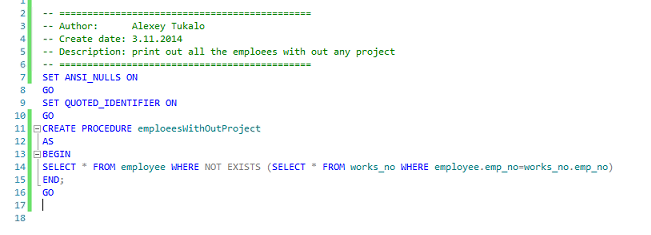
\includegraphics[scale=.9]{ProcedureSQL/firstProcedureSource}}
\caption{The first procedure source code}
\end{figure}\\
The code should display employees with out any project. The employees and projects tables are shown on the picture 2.
\begin{figure}[hb]
\centerline{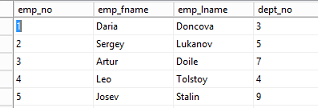
\includegraphics{ProcedureSQL/emploee}}\vspace{0.1in}
\centerline{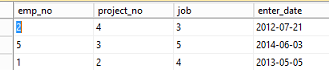
\includegraphics{ProcedureSQL/projects}}
\caption{The employees and projects tables}
\end{figure}\\
And the output of the procedure is below.
\begin{figure}[hb]
\centerline{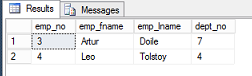
\includegraphics{ProcedureSQL/output1}}
\caption{The employees  without any project}
\end{figure}

\section{Increase all the project budgets with a \%-value given as a parameter}
After that I have made the second procedure the source code you can see at the pic. 4.
\begin{figure}[H]
\centerline{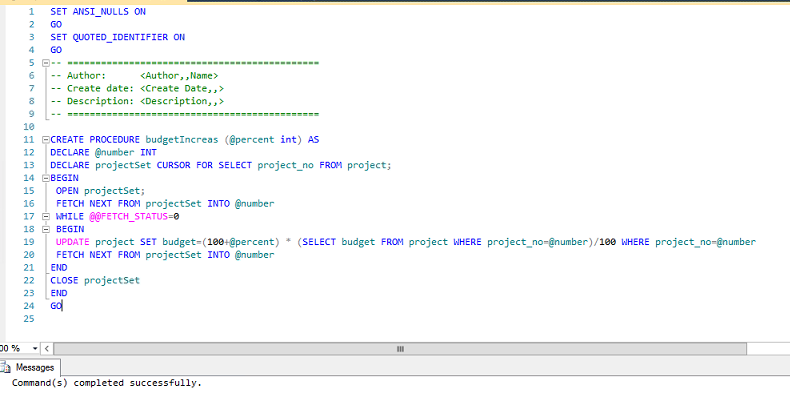
\includegraphics[scale=0.8]{ProcedureSQL/secondeProcedureSource}}
\caption{budgetIncreas() source code}
\end{figure}
The budgets before the execution was at figure 5.
\begin{figure}[H]
\centerline{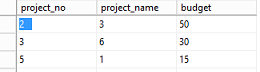
\includegraphics[scale=0.8]{ProcedureSQL/budgetBeffor}}
\caption{budgets before the execution}
\end{figure}
I have made the execution via GUI tools.  
\begin{figure}[H]
\centerline{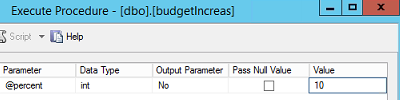
\includegraphics[scale=0.8]{ProcedureSQL/executionbudget}}
\caption{Execution settings}
\end{figure}
And finally I got the new budgets.
\begin{figure}[H]
\centerline{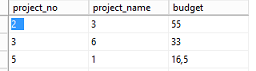
\includegraphics[scale=0.8]{ProcedureSQL/budgetAfter}}
\caption{Execution settings}
\end{figure}
\section{Archive orders}
I needed to write a procedure to move all old orders to special table for an archive, the procedure is shown below.
\begin{figure}[H]
\centerline{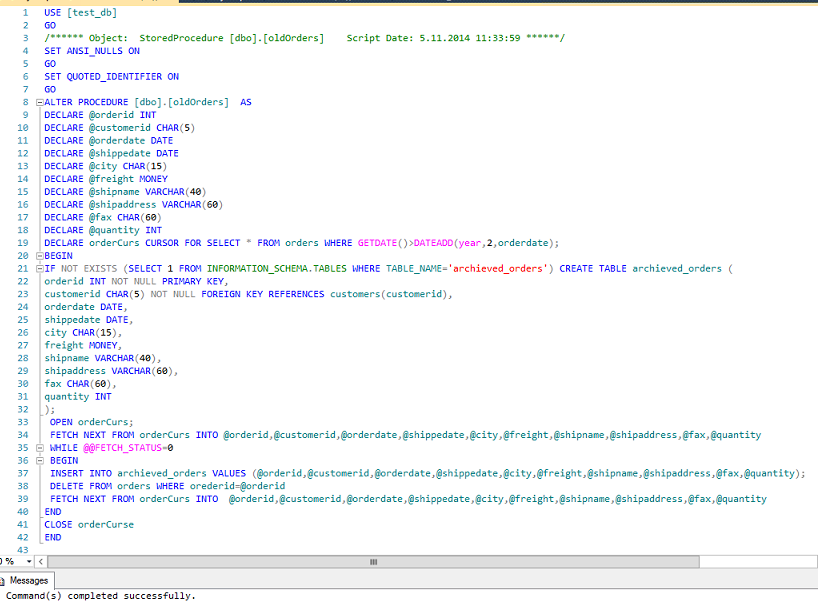
\includegraphics[scale=0.8]{ProcedureSQL/thirdSourceCOde}}
\caption{The third procedure}
\end{figure}
The orders table before execution is shown on the pic below.  
\begin{figure}[H]
\centerline{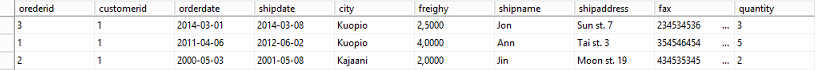
\includegraphics[scale=0.8]{ProcedureSQL/orders}}
\caption{Orders before the procedure execution}
\end{figure}
After the execution I have got two table pic. 10. The first table shows as the archived orders and the second one current.
\begin{figure}[H]
\centerline{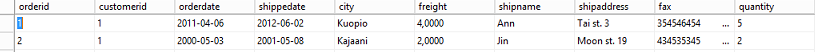
\includegraphics[scale=0.8]{ProcedureSQL/arc_orders}}
\centerline{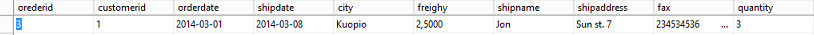
\includegraphics[scale=0.8]{ProcedureSQL/ordersafter}}
\caption{Archived\_orders and orders table after the procedure execution}
\end{figure}

\end{document}
